So far we have introduced the QAC language family for representing servers and
validators, and demonstrated the derivation mechanism with a $\Prog$ language.
Next I'll show how to prove that QAC validators are sound and complete:
\[\begin{array}{r@{\;}l}
\forall p:\Prog,&\letin{s}{\serverOf(p)}\\
&\letin{v}{\validatorOf(p)}\\
&\rejSound v s\wedge\rejComplete v s\\
&\text{\it i.e. }\forall t:\List(Q\times A),\\
&\qquad\valid s t\iff\accepts v t\\
&\qquad\text{\it i.e. }\exists s',\behaves s t s'\iff\exists v',\behaves v t v'
\end{array}\]

This section first presents a generic framework for proving validators'
correctness properties, and then demonstrates its usage by applying it to
$\Prog$-based validators.

\subsection{Proof strategy}
Both the specification and the validator are infinite loops, and the correctness
property is defined as equivalence between production and consumption of traces.
Therefore, we can prove this bisimulation relation by introducing some loop
invariant, and show that it is preserved in each step between the specification
and the validator.

\paragraph{Rejection soundness (acceptance completeness)}
To prove that any trace producible by server $\existT{S}{\sigma}{(\sstep,s_0)}$
is consumable by validator $\existT{V}{\beta}{(\vstep,v_0)}$, we need forward
induction on the server's execution path, and show that every step has a
corresponding validator step:
\begin{itemize}
\item The initial server state $s_0$ reflects the initial validator state $v_0$:
  \begin{equation}
    \tag{RejSound1}
    \label{eq:rs1}
    \Reflects{(v_0:\beta)}{(s_0:\sigma)}
  \end{equation}
\item Any server step $\sstep(q,c,s)=(a,s')$ whose pre-execution state $s$
  reflects some pre-validation state $v$ can be consumed by the validator
  into a post-validation state $v'$ that reflects the post-execution state $s'$:
  \begin{align*}
    \tag{RejSound2}
    \label{eq:rs2}
    &\forall(q:Q)(c:C)(a:A)(s,s':\sigma)(v:\beta),\\
    &\sstep(q,c,s)=(a,s')\wedge\Reflects{v}{s}\\
    &\implies\exists v':\beta,\vstep(q,a,v)=\Some{v'}\wedge\Reflects{v'}{s'}
  \end{align*}
  \begin{center}
    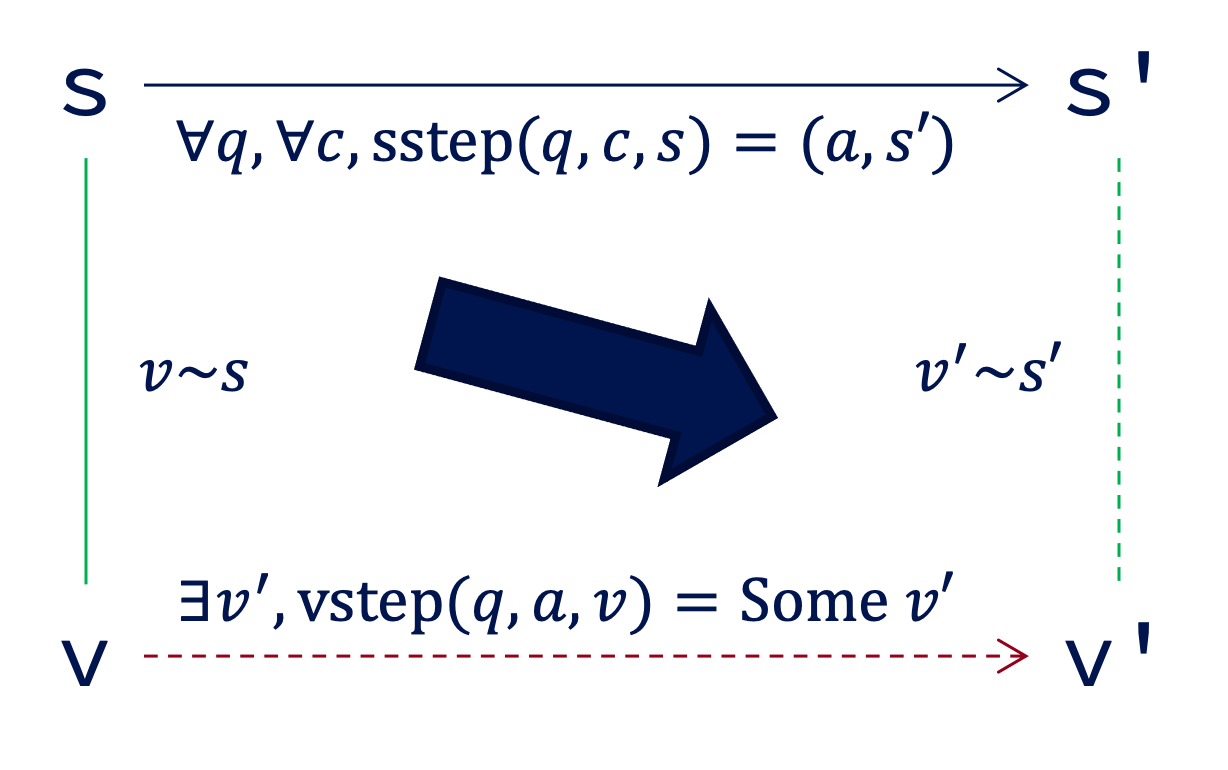
\includegraphics[width=.5\textwidth]{figures/sound}
  \end{center}
\end{itemize}

\paragraph{Rejection completeness (acceptance soundness)}
To prove that any trace consumable by validator
$\existT{V}{\beta}{(\vstep,v_0)}$ is producible by server
$\existT{S}{\sigma}{(\sstep,s_0)}$, we need backward induction on the
validator's execution path, and show that every step has a corresponding server
step:
\begin{itemize}
\item Any accepting validator step $\vstep(q,a,v)=\Some v'$ has some server
  state $s'$ that reflects the post-validation state $v'$:
  \begin{align*}
    \tag{RejComplete1}
    \label{eq:rc1}
    \forall(q:Q)(a:A)(v, v':\beta),\;&\vstep(q,a,v)=\Some{v'}\\
    &\implies\exists s':\sigma,\Reflects{v'}{s'} 
  \end{align*}
\item Any accepting validator step $\vstep(q,a,v)=\Some v'$ whose
  post-validation state $v'$ reflects some post-execution server state $s'$
  has a corresponding server step from a pre-execution state $s$
  that reflects the pre-validation state $v$:
  \begin{align*}
    \tag{RejComplete2}
    \label{eq:rc2}
    &\forall(q:Q)(a:A)(v,v':\beta)(s':\sigma),\\
    &\vstep(q,a,v)=\Some{v'}\wedge\Reflects{v'}{s'}\\
    &\implies\exists(s:\sigma)(c:C),\sstep(q,c,s)=(a,s')\wedge\Reflects{v}{s}
  \end{align*}
  \begin{center}
    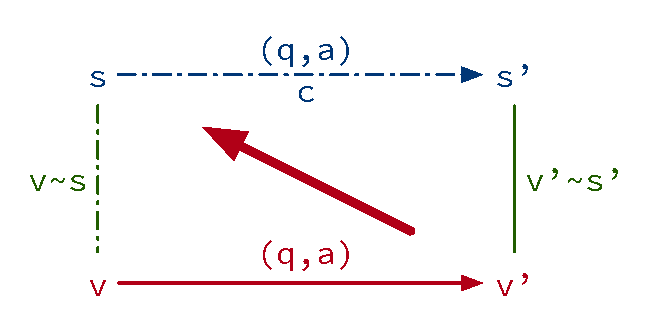
\includegraphics[width=.5\textwidth]{figures/complete}
  \end{center}

\item The initial validator state $v_0$ only reflects the initial server state $s_0$:
  \begin{equation}
    \tag{RejComplete3}
    \label{eq:rc3}
    \{s\mid\Reflects{v_0}{s}\}=\{s_0\}
  \end{equation}
\end{itemize}

Rejection soundness is proven by forward induction, while rejection completeness
is proven by backward induction.  This is because the choice $C$ is known from
the server step, but unknown from the validator step: Given a validator step, we
cannot predict ``what choices the server will make in the future'', but can
analyze ``what choices the server might have made in the past''.  This proof
strategy is further explained with the $\Prog$ example.

\subsection{Case study: Proving $\Prog$-based validators' correctness}
For specifications written in the $\Prog$ language, the validator is derived by
dualizing the server model.  It maintains a set of validation states, each state
corresponds to a possible execution path of the model program.

A validation state is accepting if its constraints are satisfiable, {\it i.e.}
there exists an assignment of the symbolic variables that can unify the trace
with the server model.

The validator accepts the trace if any of its validation states is accepting,
which indicates that some execution path of the server model can produce the
trace.

Given an accepting validation state, we can construct the server steps that
produce the trace, using the assignment $(\Var\to\Int)$ that satisfies the
constraints.  This assignment evaluates internal choices' symbolic variables
into concrete values, and evaluates the validator's key-variable mapping
$(\Nat\to\Var)$ to the server's key-value mapping $(\Nat\to\Int)$.

Therefore, we only need to show that each server and validator step preserves
the existence of such assignment that relates their states.

For the rest of this section, $\beta=\Set((\Nat\to\Var)\times\Set\constraint)$
represents the validator state type, and $\sigma=\Nat\to\Int$ represents the
server state type.

\begin{definition}[Invariant between $\Prog$-based specification and validator]
  Validator state $v$ {\em simulates} server state $s$ if it contains a
  validation state $(vs,cs)$ that {\em reflects} the server state, {\it i.e.}
  (1) There exists an assignment $asgn$ that can satisfy the constraints $cs$;
  and (2) The key-variable mapping $vs$ can be evaluated with $asgn$ (written as
  $vs^{asgn}$) into a key-value mapping that is equivalent with
  $s$:
  \[\begin{array}{lll} \Reflects{(v:\beta)}{(s:\sigma)}&\triangleq&
  \exists((vs,cs)\in v)(asgn:\Var\to\Int),\satisfy{asgn} cs\wedge vs^{asgn}\equiv s\\
  vs^{asgn}&\triangleq&addr\mapsto asgn!(vs!addr) \end{array}\]
\end{definition}

\begin{lemma}[\ref{eq:rs1}]
\[\begin{array}{ll}
\text{If:}&
vs=(\_\mapsto\#0)\qquad
cs=\{\#0\equiv0\}\qquad
s=(\_\mapsto0)\\
\text{Then:}&\Reflects{\{(vs,cs)\}}{s}
\end{array}\]
\end{lemma}
\begin{proof}
Since $(vs,cs)$ is the only element in the validator state, we only need to show
that:
\[\exists(asgn:\Var\to\Int),\satisfy{asgn} cs\wedge vs^{asgn}\equiv s\]

By constructing the assignment as: \[asgn=(\_\mapsto0)\]

We have: \[\#0^{asgn}\equiv0\]

Thus: \[\satisfy{asgn} cs\]

We also know that: \[\forall addr, asgn!(vs!addr)=0\equiv s!addr)\]

Thus: \[(vs^{asgn}\equiv s)\]
\end{proof}

\begin{lemma}[\ref{eq:rs2}]
  \begin{align*}
    &\forall(p:\Prog)(q,c,a:\Int)(s_0,s':\sigma)(v:\beta),\\
    &\sstep_p(q,c,s_0)=(a,s')\wedge\Reflects{v}{s_0}\\
    &\implies\exists v':\beta,\vstep_p(q,a,v)=\Some{v'}\wedge\Reflects{v'}{s'}
  \end{align*}
\end{lemma}
\begin{proof}
The invariant $\Reflects{v}{s_0}$ tells us that $v$ contains a validation state
that reflects the server state $s_0$:
\[\exists((vs_0,cs_0)\in v)(asgn_0:\Var\to\Int),\satisfy{asgn_0} cs_0\wedge {vs_0}^{asgn_0}\equiv s_0\]

The corresponding validator step is constructed by analyzing the server step,
and proving small-step bisimulation for each derivation rule
in \autoref{sec:dualization}.
\begin{enumerate}
\item The server first writes the internal choice $c$ to address $!1$.
According to \autoref{rule:choice}, the validator creates a fresh variable for
address $!1$.

We need to show that:
\[\exists asgn_1,\satisfy{asgn_1} cs_0\wedge vs_1^{asgn_1}\equiv s_1\]

\begin{proof}
We can construct the following assignment:
\[asgn_1=\update{asgn_0}{x_c}{c}\]

Since $x_c$ is fresh in $cs_0$, we have:
\[\forall (e_1\ccmp e_2)\in cs_0,{e_1}^{asgn_1}={e_1}^{asgn_0}\wedge{e_2}^{asgn_1}={e_2}^{asgn_0}\]

Thus:
\begin{align*}
&\forall (e_1\ccmp e_2)\in cs_0, {e_1}^{asgn_1}\ccmp {e_2}^{asgn_1}\\
&\textit{i.e. }\satisfy{asgn_1} cs_0
\end{align*}

Since $x_c$ is also fresh in $vs_0$, we have:
\[\forall addr, asgn_1!(vs_1!addr)=\begin{cases}
asgn_1!x_c=c\equiv s_1!addr&addr\Is1\\
asgn_0!(vs_0!addr)=s_0!addr\equiv s_1!addr&\text{otherwise}
\end{cases}\]

Thus: \[{vs_1}^{asgn_1}\equiv s_1\]
\end{proof}

\item When the server writes some expression $(e:\Sexp)$ to an address $!dst$,
the validator creates a fresh variable $x_e$ for address $!dst$, and constraints
that $\#x_e\equiv e^{vs},$\footnote{If unspecified, $(vs,cs)$ represents the
validator state at the current point of derivation, and $s$ represents the
current server state.} according to \autoref{rule:write}.

We need to show that:
\begin{align*}
\forall vs,cs,s,asgn,&\satisfy{asgn}{cs}\wedge vs^{asgn}\equiv s\\
&\implies\forall d,e,\letin{}{}
\end{align*}
\end{enumerate}

\end{proof}

This bisimulation definition satisfies the hypotheses for proving soundness and
completeness:

Hypotheses~\ref{eq:rs1} and \ref{eq:rc3} are immediate from the initial states'
definition: The initial server state is all-zero map.  The initial validator
state is a singleton that maps all addresses to a variable that is constrained
to have value zero.

\autoref{eq:rc1} is based on the fact that $\vstep_p$ checks the nonemptiness of
the result:
\[\forall q~a~v~v',\vstep_p(q,a,v)=\Some{v'}\implies(\vstep_p'(q,a,v)=v'\wedge\exists (vs,cs)\in v')\]
and that $\vstep_p'$ guards the satisfiability of all constraints in its result:
\[\forall q~a~vs~cs,{(vs,cs)}\in\vstep_p'(q,a,v)\implies\exists asgn,\satisfy{asgn}cs\]

Therefore, any element in the resulting validator state can construct a
simulating server state:
\[\forall asgn~cs~vs~v,(\satisfy{asgn}cs\wedge(vs,cs)\in v)\implies \Reflects{v}{vs^{asgn}}\]

\autoref{eq:rs2} is based on the fact that the pre-validation state must contain
an element that reflects the server's pre-execution state, as defined by the
bisimulation relation.  Given the server's internal choices, we can compute its
execution path.  By induction on the server's execution path, we can construct
the corresponding post-validation state by making the same internal choice and
branch decisions as the server did, and construct the assignment that satisfies
the validator's constraints.

\autoref{eq:rc3} observes that validator design increases the constraints
monotonically.  Therefore, ``assignments that can satisfy the post-validation
constraints'' is a subset of ``assignments that can satisfy the pre-validation
constraints'':
\[\forall q~a~vs~cs~vs'~cs'~asgn,((vs',cs')\in\vstep_p'(q,a,(vs,cs))\wedge\satisfy{asgn} cs')\implies\satisfy{asgn}cs\]

As a result, the corresponding pre-step server state and the internal choice can
be constructed, and proven to perform the server-side step:
\begin{align*}
\forall q~a~vs~cs~vs'~cs'~asgn,\;&(vs',cs')\in\vstep_p'(q,a,(vs,cs))\\
&\implies\sstep_p(q,asgn!(\Fresh{vs}),vs^{asgn})=vs'^{~asgn}
\end{align*}

The intuition here is that the assignment includes ``all choices made by the
server, past and future'', which is narrowed upon more and more observations.
Therefore, the assignment can instantiate all previous validator states into
corresponding servers, and reconstruct the server's execution path by inferring
its internal choices.
